% Diagrammi di sequenza (sezione Interaction del report).
% Sorgente TikZ autonomo come gli altri: ogni tikzpicture è una PAGINA del
% PDF e il report sceglie il diagramma con \includegraphics[page=N].
%   cd doc/figures && latexmk -pdf diagrammi-sequenza.tex && latexmk -c diagrammi-sequenza.tex
% Pagine: 1 login + idratazione + presenza, 2 claim, 3 resolve, 4 escalation.
% Ogni diagramma ha DUE pod api, perché il punto è mostrare cosa attraversa
% i pod (Redis Pub/Sub) e cosa no (Change Stream, uno per pod). Messaggi,
% chiavi e codici di risposta vanno tenuti allineati a api/src.
\documentclass[tikz,border=3pt]{standalone}
\usepackage[T1]{fontenc}
\usepackage{lmodern}
\usepackage{amssymb}
\usetikzlibrary{arrows.meta,calc}

\definecolor{edge}{HTML}{3B4252}
\definecolor{muted}{HTML}{5F6672}
\definecolor{netfill}{HTML}{E8EEF7}   \definecolor{netline}{HTML}{3A5A8C}
\definecolor{apifill}{HTML}{EEF0FA}   \definecolor{apiline}{HTML}{4B55A0}
\definecolor{redfill}{HTML}{FBECEA}   \definecolor{redline}{HTML}{A3402F}
\definecolor{mgofill}{HTML}{EAF4F1}   \definecolor{mgoline}{HTML}{2F7564}
\definecolor{fragline}{HTML}{8A8F99}

\tikzset{
  font=\sffamily\scriptsize,
  part/.style={draw=#1line, fill=#1fill, line width=0.8pt, rounded corners=2pt,
               align=center, minimum width=2.05cm, minimum height=0.75cm,
               font=\sffamily\footnotesize, inner sep=2pt},
  life/.style={draw=muted, dash pattern=on 2pt off 1.5pt, line width=0.5pt},
  call/.style={->, >={Stealth[length=2mm,width=1.5mm]}, draw=edge, line width=0.65pt},
  ret/.style={->, >={Stealth[open,length=2mm,width=1.5mm]}, draw=edge, line width=0.55pt,
              dash pattern=on 2.5pt off 1.5pt},
  async/.style={->, >={Straight Barb[length=2mm,width=2mm]}, draw=edge, line width=0.65pt},
  mlab/.style={font=\sffamily\scriptsize, text=edge, inner sep=1pt, fill=white,
               fill opacity=0.9, text opacity=1, align=center},
  frag/.style={draw=fragline, line width=0.6pt},
  ftag/.style={draw=fragline, fill=white, font=\sffamily\scriptsize\bfseries, text=edge,
               inner sep=2pt, anchor=north west},
  guard/.style={font=\sffamily\scriptsize\itshape, text=edge, inner sep=1.5pt, anchor=north west},
  note/.style={draw=muted!60, fill=yellow!8, font=\sffamily\scriptsize, text=edge,
               align=left, inner sep=2pt},
}

% Partecipanti: la x di ognuno viene salvata per i messaggi.
\makeatletter
\newcommand{\participant}[4]{% id, x, etichetta, colore
  \expandafter\def\csname lx@#1\endcsname{#2}%
  \node[part=#4] (#1) at (#2,0) {#3};}
\newcommand{\lx}[1]{\csname lx@#1\endcsname}
\makeatother
\newcommand{\lifelines}[2]{% elenco di id, y finale
  \foreach \p in {#1} {\draw[life] (\p.south) -- (\lx{\p},#2);}}
% Messaggi: \msg[stile]{da}{a}{y}{etichetta}
% L'etichetta parte dall'estremo sinistro della freccia: in un diagramma
% di sequenza si legge da sinistra, e così non sporge oltre il primo pod.
\newcommand{\msg}[5][call]{%
  \pgfmathsetmacro\xmin{min(\lx{#2},\lx{#3})}%
  \draw[#1] (\lx{#2},#4) -- (\lx{#3},#4);
  \node[mlab, anchor=south west] at (\xmin+0.08,#4+0.02) {#5};}
% Messaggio con etichetta su due righe, sopra e sotto la freccia.
\newcommand{\msgtwo}[5]{% da, a, y, riga sopra, riga sotto
  \pgfmathsetmacro\xmin{min(\lx{#1},\lx{#2})}%
  \draw[call] (\lx{#1},#3) -- (\lx{#2},#3);
  \node[mlab, anchor=south west] at (\xmin+0.08,#3+0.02) {#4};
  \node[mlab, anchor=north west] at (\xmin+0.08,#3-0.04) {#5};}
% Messaggio verso se stessi (elaborazione locale).
\newcommand{\selfmsg}[3]{% id, y, etichetta
  \draw[call] (\lx{#1},#2) -- ++(0.35,0) -- ++(0,-0.32) -- ++(-0.35,0);
  \node[mlab, anchor=west] at ($(\lx{#1},#2)+(0.4,-0.16)$) {#3};}
% Frammenti combinati: \fragment{op}{xl}{xr}{ytop}{ybot}{guardia}
\newcommand{\fragment}[6]{%
  \draw[frag] (#2,#4) rectangle (#3,#5);
  \node[ftag] (ft) at (#2,#4) {#1};
  \node[guard] at ($(ft.north east)+(0.05,0)$) {#6};}
\newcommand{\fragsep}[4]{% xl, xr, y, guardia
  \draw[frag, dash pattern=on 3pt off 2pt] (#1,#3) -- (#2,#3);
  \node[guard] at (#1,#3) {#4};}

\begin{document}

% =====================================================================
% 1. Login, handshake, presenza e idratazione
% =====================================================================
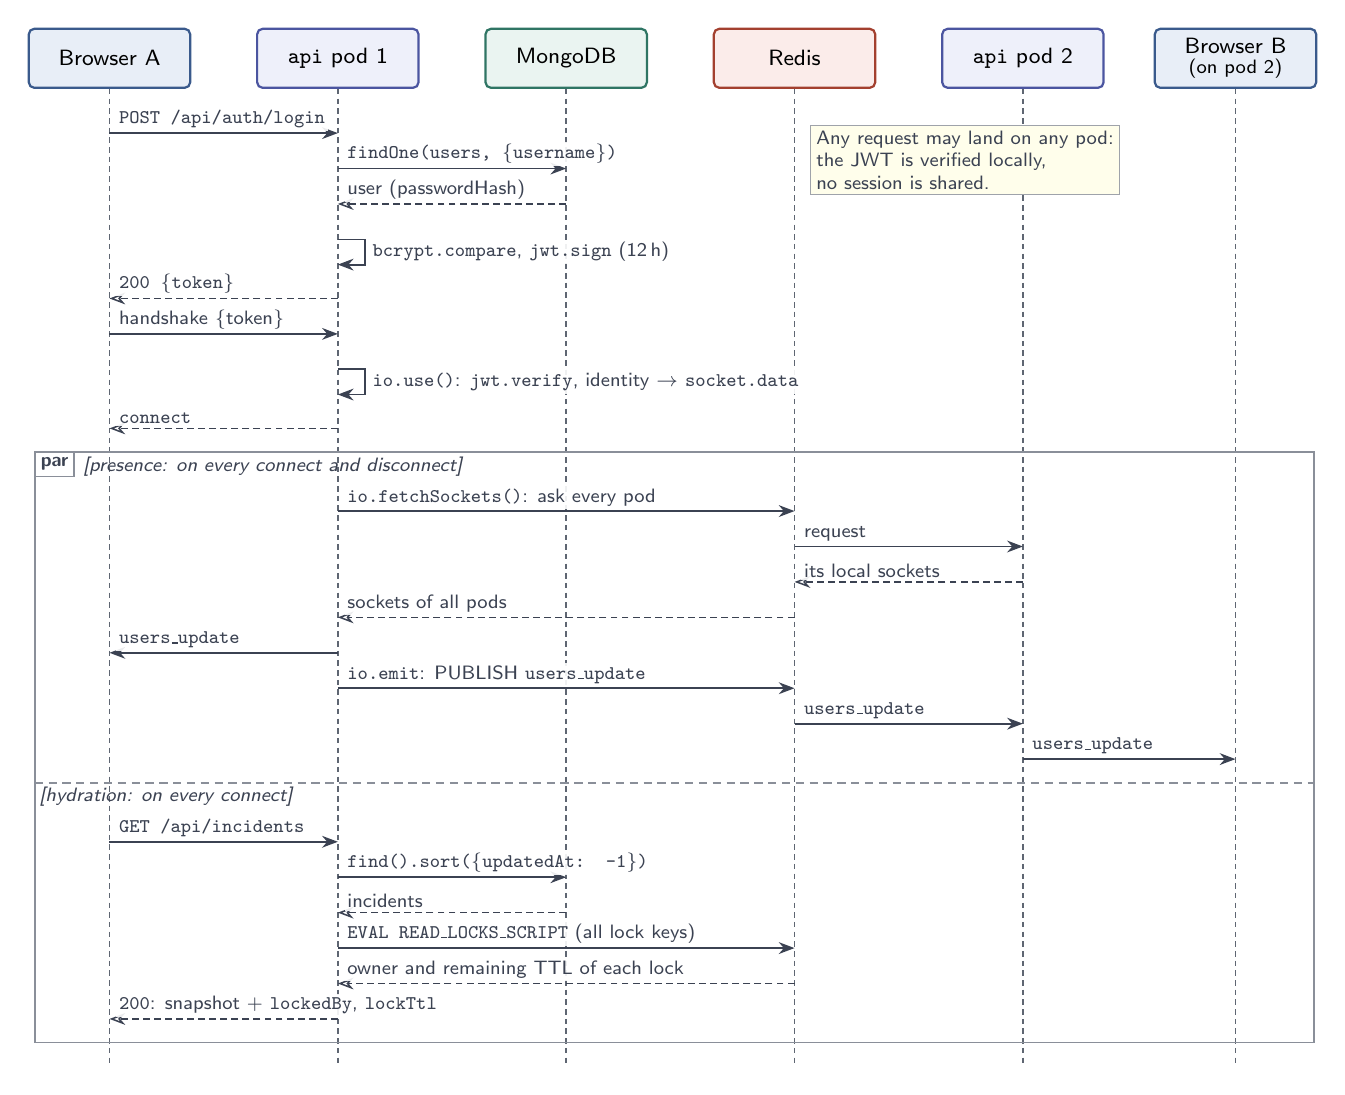
\begin{tikzpicture}
\participant{A}{0}{Browser A}{net}
\participant{P1}{2.9}{\texttt{api} pod 1}{api}
\participant{M}{5.8}{MongoDB}{mgo}
\participant{R}{8.7}{Redis}{red}
\participant{P2}{11.6}{\texttt{api} pod 2}{api}
\participant{B}{14.3}{Browser B\\[-2pt]{\scriptsize(on pod 2)}}{net}
\lifelines{A,P1,M,R,P2,B}{-12.8}

\msg{A}{P1}{-0.95}{\texttt{POST /api/auth/login}}
\msg{P1}{M}{-1.4}{\texttt{findOne(users, \{username\})}}
\msg[ret]{M}{P1}{-1.85}{user (passwordHash)}
\selfmsg{P1}{-2.3}{\texttt{bcrypt.compare}, \texttt{jwt.sign} (12\,h)}
\msg[ret]{P1}{A}{-3.05}{\texttt{200 \{token\}}}
\msg{A}{P1}{-3.5}{handshake \{token\}}
\selfmsg{P1}{-3.95}{\texttt{io.use()}: \texttt{jwt.verify}, identity $\to$ \texttt{socket.data}}
\msg[ret]{P1}{A}{-4.7}{\texttt{connect}}

\fragment{par}{-0.95}{15.3}{-5.0}{-12.5}{[presence: on every connect and disconnect]}
\msg{P1}{R}{-5.75}{\texttt{io.fetchSockets()}: ask every pod}
\msg{R}{P2}{-6.2}{request}
\msg[ret]{P2}{R}{-6.65}{its local sockets}
\msg[ret]{R}{P1}{-7.1}{sockets of all pods}
\msg{P1}{A}{-7.55}{\texttt{users\_update}}
\msg{P1}{R}{-8.0}{\texttt{io.emit}: PUBLISH \texttt{users\_update}}
\msg{R}{P2}{-8.45}{\texttt{users\_update}}
\msg{P2}{B}{-8.9}{\texttt{users\_update}}
\fragsep{-0.95}{15.3}{-9.2}{[hydration: on every connect]}
\msg{A}{P1}{-9.95}{\texttt{GET /api/incidents}}
\msg{P1}{M}{-10.4}{\texttt{find().sort(\{updatedAt: -1\})}}
\msg[ret]{M}{P1}{-10.85}{incidents}
\msg{P1}{R}{-11.3}{\texttt{EVAL READ\_LOCKS\_SCRIPT} (all lock keys)}
\msg[ret]{R}{P1}{-11.75}{owner and remaining TTL of each lock}
\msg[ret]{P1}{A}{-12.2}{\texttt{200}: snapshot + \texttt{lockedBy}, \texttt{lockTtl}}

\node[note, anchor=north west] at (8.9,-0.85) {Any request may land on any pod:\\the JWT is verified locally,\\no session is shared.};
\end{tikzpicture}

% =====================================================================
% 2. Claim di un incidente
% =====================================================================
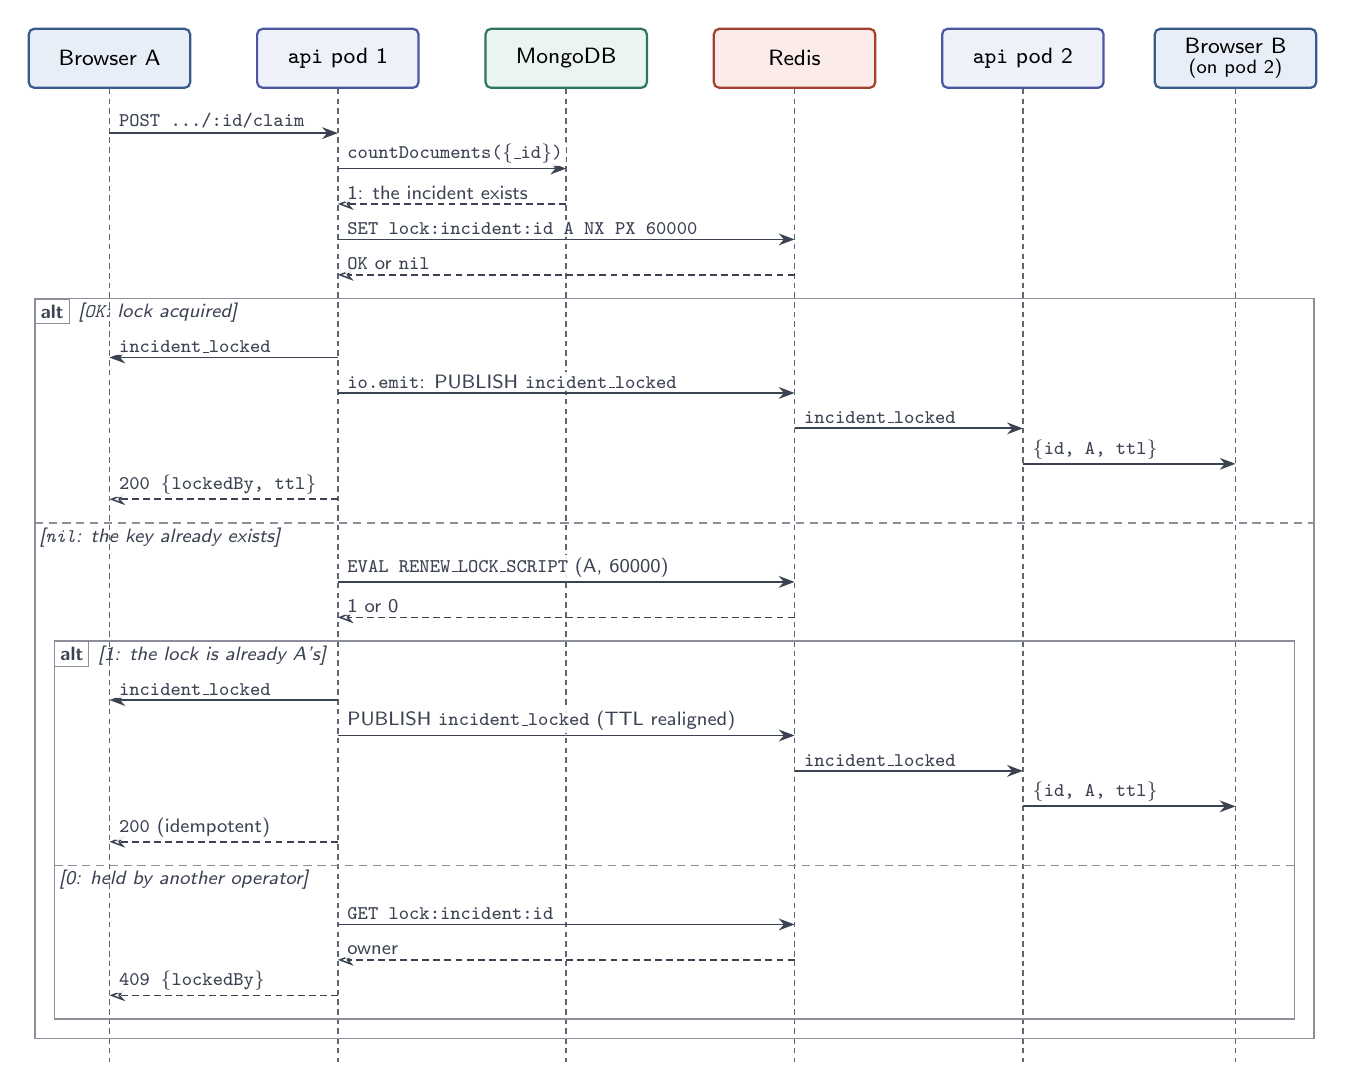
\begin{tikzpicture}
\participant{A}{0}{Browser A}{net}
\participant{P1}{2.9}{\texttt{api} pod 1}{api}
\participant{M}{5.8}{MongoDB}{mgo}
\participant{R}{8.7}{Redis}{red}
\participant{P2}{11.6}{\texttt{api} pod 2}{api}
\participant{B}{14.3}{Browser B\\[-2pt]{\scriptsize(on pod 2)}}{net}
\lifelines{A,P1,M,R,P2,B}{-12.75}

\msg{A}{P1}{-0.95}{\texttt{POST .../:id/claim}}
\msg{P1}{M}{-1.4}{\texttt{countDocuments(\{\_id\})}}
\msg[ret]{M}{P1}{-1.85}{1: the incident exists}
\msg{P1}{R}{-2.3}{\texttt{SET lock:incident:id A NX PX 60000}}
\msg[ret]{R}{P1}{-2.75}{\texttt{OK} or \texttt{nil}}

\fragment{alt}{-0.95}{15.3}{-3.05}{-12.45}{[\texttt{OK}: lock acquired]}
\msg{P1}{A}{-3.8}{\texttt{incident\_locked}}
\msg{P1}{R}{-4.25}{\texttt{io.emit}: PUBLISH \texttt{incident\_locked}}
\msg{R}{P2}{-4.7}{\texttt{incident\_locked}}
\msg{P2}{B}{-5.15}{\texttt{\{id, A, ttl\}}}
\msg[ret]{P1}{A}{-5.6}{\texttt{200 \{lockedBy, ttl\}}}
\fragsep{-0.95}{15.3}{-5.9}{[\texttt{nil}: the key already exists]}
\msg{P1}{R}{-6.65}{\texttt{EVAL RENEW\_LOCK\_SCRIPT} (A, 60000)}
\msg[ret]{R}{P1}{-7.1}{1 or 0}
\fragment{alt}{-0.7}{15.05}{-7.4}{-12.2}{[1: the lock is already A's]}
\msg{P1}{A}{-8.15}{\texttt{incident\_locked}}
\msg{P1}{R}{-8.6}{PUBLISH \texttt{incident\_locked} (TTL realigned)}
\msg{R}{P2}{-9.05}{\texttt{incident\_locked}}
\msg{P2}{B}{-9.5}{\texttt{\{id, A, ttl\}}}
\msg[ret]{P1}{A}{-9.95}{\texttt{200} (idempotent)}
\fragsep{-0.7}{15.05}{-10.25}{[0: held by another operator]}
\msg{P1}{R}{-11.0}{\texttt{GET lock:incident:id}}
\msg[ret]{R}{P1}{-11.45}{owner}
\msg[ret]{P1}{A}{-11.9}{\texttt{409 \{lockedBy\}}}
\end{tikzpicture}

% =====================================================================
% 3. Risoluzione: due canali in parallelo
% =====================================================================
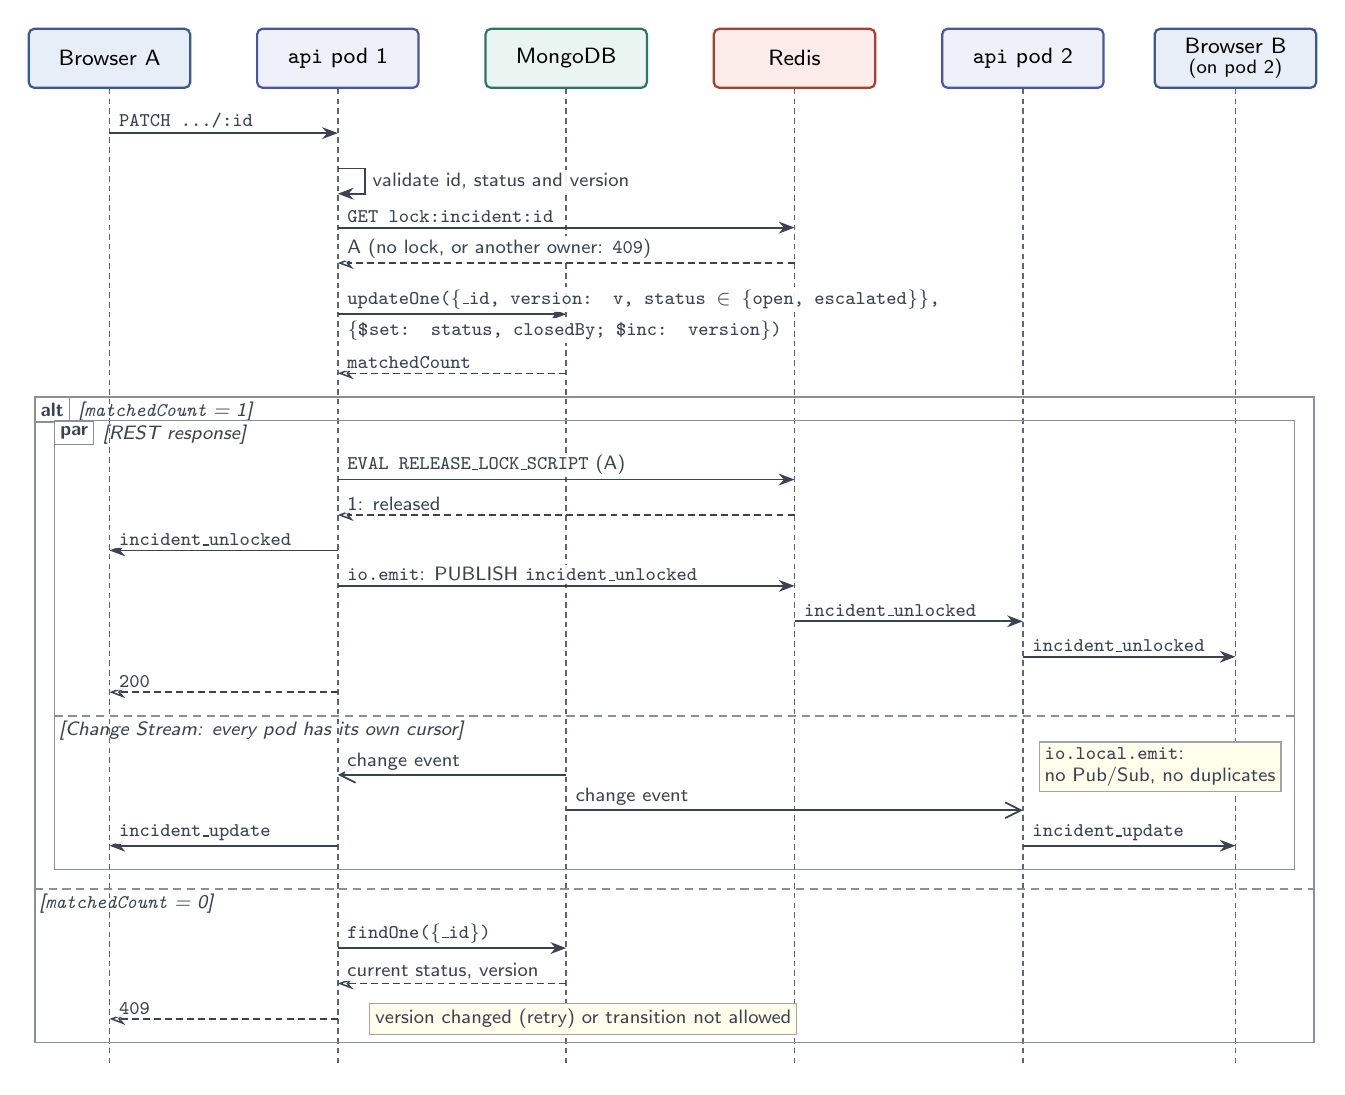
\begin{tikzpicture}
\participant{A}{0}{Browser A}{net}
\participant{P1}{2.9}{\texttt{api} pod 1}{api}
\participant{M}{5.8}{MongoDB}{mgo}
\participant{R}{8.7}{Redis}{red}
\participant{P2}{11.6}{\texttt{api} pod 2}{api}
\participant{B}{14.3}{Browser B\\[-2pt]{\scriptsize(on pod 2)}}{net}
\lifelines{A,P1,M,R,P2,B}{-12.8}

\msg{A}{P1}{-0.95}{\texttt{PATCH .../:id}}
\selfmsg{P1}{-1.4}{validate id, status and version}
\msg{P1}{R}{-2.15}{\texttt{GET lock:incident:id}}
\msg[ret]{R}{P1}{-2.6}{A (no lock, or another owner: \texttt{409})}
\msgtwo{P1}{M}{-3.25}{\texttt{updateOne(\{\_id, version: v, status $\in$ \{open, escalated\}\},}}{\texttt{\{\$set: status, closedBy; \$inc: version\})}}
\msg[ret]{M}{P1}{-4.0}{\texttt{matchedCount}}

\fragment{alt}{-0.95}{15.3}{-4.3}{-12.5}{[\texttt{matchedCount} = 1]}
\fragment{par}{-0.7}{15.05}{-4.6}{-10.3}{[REST response]}
\msg{P1}{R}{-5.35}{\texttt{EVAL RELEASE\_LOCK\_SCRIPT} (A)}
\msg[ret]{R}{P1}{-5.8}{1: released}
\msg{P1}{A}{-6.25}{\texttt{incident\_unlocked}}
\msg{P1}{R}{-6.7}{\texttt{io.emit}: PUBLISH \texttt{incident\_unlocked}}
\msg{R}{P2}{-7.15}{\texttt{incident\_unlocked}}
\msg{P2}{B}{-7.6}{\texttt{incident\_unlocked}}
\msg[ret]{P1}{A}{-8.05}{\texttt{200}}
\fragsep{-0.7}{15.05}{-8.35}{[Change Stream: every pod has its own cursor]}
\msg[async]{M}{P1}{-9.1}{change event}
\msg[async]{M}{P2}{-9.55}{change event}
\msg{P1}{A}{-10.0}{\texttt{incident\_update}}
\msg{P2}{B}{-10.0}{\texttt{incident\_update}}
\fragsep{-0.95}{15.3}{-10.55}{[\texttt{matchedCount} = 0]}
\msg{P1}{M}{-11.3}{\texttt{findOne(\{\_id\})}}
\msg[ret]{M}{P1}{-11.75}{current status, version}
\msg[ret]{P1}{A}{-12.2}{\texttt{409}}

\node[note, anchor=west] at (11.8,-9.0) {\texttt{io.local.emit}:\\no Pub/Sub, no duplicates};
\node[note, anchor=west] at (3.3,-12.2) {version changed (retry) or transition not allowed};
\end{tikzpicture}

% =====================================================================
% 4. Escalation SLA eseguita dal leader
% =====================================================================
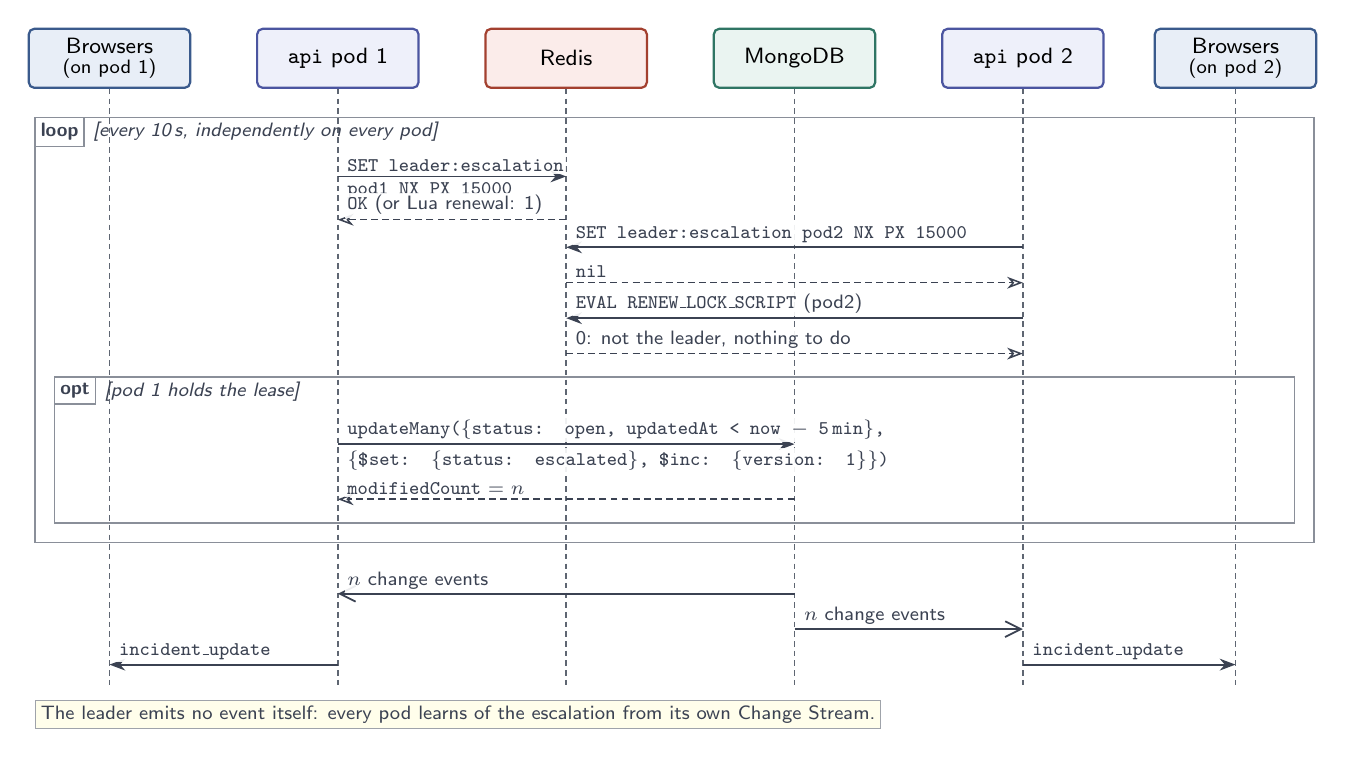
\begin{tikzpicture}
\participant{A}{0}{Browsers\\[-2pt]{\scriptsize(on pod 1)}}{net}
\participant{P1}{2.9}{\texttt{api} pod 1}{api}
\participant{R}{5.8}{Redis}{red}
\participant{M}{8.7}{MongoDB}{mgo}
\participant{P2}{11.6}{\texttt{api} pod 2}{api}
\participant{B}{14.3}{Browsers\\[-2pt]{\scriptsize(on pod 2)}}{net}
\lifelines{A,P1,R,M,P2,B}{-8.0}

\fragment{loop}{-0.95}{15.3}{-0.75}{-6.15}{[every 10\,s, independently on every pod]}
\msgtwo{P1}{R}{-1.5}{\texttt{SET leader:escalation}}{\texttt{pod1 NX PX 15000}}
\msg[ret]{R}{P1}{-2.05}{\texttt{OK} (or Lua renewal: 1)}
\msg{P2}{R}{-2.4}{\texttt{SET leader:escalation pod2 NX PX 15000}}
\msg[ret]{R}{P2}{-2.85}{\texttt{nil}}
\msg{P2}{R}{-3.3}{\texttt{EVAL RENEW\_LOCK\_SCRIPT} (pod2)}
\msg[ret]{R}{P2}{-3.75}{0: not the leader, nothing to do}
\fragment{opt}{-0.7}{15.05}{-4.05}{-5.9}{[pod 1 holds the lease]}
\msgtwo{P1}{M}{-4.9}{\texttt{updateMany(\{status: open, updatedAt < now $-$ 5\,min\},}}{\texttt{\{\$set: \{status: escalated\}, \$inc: \{version: 1\}\})}}
\msg[ret]{M}{P1}{-5.6}{\texttt{modifiedCount} = $n$}

\msg[async]{M}{P1}{-6.8}{$n$ change events}
\msg[async]{M}{P2}{-7.25}{$n$ change events}
\msg{P1}{A}{-7.7}{\texttt{incident\_update}}
\msg{P2}{B}{-7.7}{\texttt{incident\_update}}
\node[note, anchor=north west] at (-0.95,-8.15) {The leader emits no event itself: every pod learns of the escalation from its own Change Stream.};
\end{tikzpicture}

\end{document}
